% !TEX encoding = UTF-8
%Koma article
\documentclass[fontsize=12pt,paper=letter,twoside]{scrartcl}

%Standard Pre-amble
\usepackage[top=4cm,bottom=4cm,left=3cm,right=3cm,asymmetric]{geometry}
%\geometry{landscape}                % Activate for for rotated page geometry
%\usepackage[parfill]{parskip}    % Begin paragraphs with an empty line rather than an indent
\usepackage[table,xcdraw]{xcolor}
\usepackage{graphicx}

\usepackage{amsmath}
\usepackage{amssymb}
\usepackage{epstopdf}
\DeclareGraphicsRule{.tif}{png}{.png}{`convert #1 `dirname #1`/`basename #1 .tif`.png}
% Listings needs package courier
\usepackage{listings} % Needs 
\usepackage{courier}

\usepackage[framemethod=TikZ]{mdframed}
\usepackage{url}

\usepackage{sty/bsymb} %% Event-B symbols
\usepackage{sty/eventB} %% REQ and ENV
\usepackage{sty/calculation}

%Maths
\usepackage{amssymb,amsmath}
\def\Fl{\mathbb{F}}
\def\Rl{\mathbb{R}}
\def\Nl{\mathbb{N}}
\def\Bl{\mathbb{B}}
\def\St{\mathbb{S}}
\newcommand{\ovr}{\upharpoonright}
\newcommand{\var}[1]{\textit{#1}}
%Useful definitions
\newcommand{\mv}[1]{\textit{m\_#1}}
\newcommand{\cv}[1]{\textit{c\_#1}}
\newcommand{\degree}[1]{^{\circ}\mathrm{#1}}
%\newcommand{\comment}[1]{{\footnotesize \quad\texttt{--}\textrm{#1}}}
\newcommand{\im}[1]{i\texttt{-\!#1}}

\usepackage[headsepline]{scrpage2}
\pagestyle{scrheadings}
\ihead[]{\small EECS4312 Report1}
\ohead[]{\small \thepage}
\cfoot[]{}
\ofoot[]{}


%%%%PVS environment%%%%%%%%%%%%%%%%%%%
\lstnewenvironment{pvs}[1][]
    {\lstset{#1,captionpos=b,language=pvs,
    mathescape=true,
    basicstyle=\small\ttfamily,
    numbers=none,
    frame=single,
    % numberstyle=\tiny\color{gray},
    % backgroundcolor=\color{lightgray},
    firstnumber=auto
    }}
    {}
 %%%%%%%%%%%%%%%%%%%%%%%%%%%%%%%%
 
%%%%Verbatim environment%%%%%%%%%%%%%%%%%%%
\lstnewenvironment{code}[1][]
    {\lstset{#1,captionpos=b,
    mathescape=true,
    basicstyle=\small\ttfamily,
    numbers=none,
    frame=single,
    % numberstyle=\tiny\color{gray},
    % backgroundcolor=\color{lightgray},
    firstnumber=auto
    }}
    {}

% \newenvironment{boxed}[1]
%    {\begin{center}
%    #1\\[1ex]
%    \begin{tabular}{|p{0.9\textwidth}|}
%    \hline\\
%    }
%    { 
%    \\\\\hline
%    \end{tabular} 
%    \end{center}
%    }
 %%%%%%%%%%%%%%%%%%%%%%%%%%%%%%%%
 
 %Text in a box
\newenvironment{textbox}
    {\begin{center}
    \begin{tabular}{|p{0.9\textwidth}|}
    \hline\\
    }
    { 
    \\\\\hline
    \end{tabular} 
    \end{center}
    }

\usepackage{hyperref}

%Highlight \hl{}
\usepackage{soul}

\usepackage{enumitem}
\newlist{mylist}{itemize}{1}
\setlist[mylist]{label=\textbullet,leftmargin=1cm,nosep}

\usepackage{multirow}

% Reduce space between figure and caption
%\usepackage{caption}
%\captionsetup[table]{font=small,skip=0pt}     %% Adjust here
%or equivalently 
\usepackage[font=small,skip=4pt]{caption}
%Useful definitions
%\newcommand{\mv}[1]{\textit{m\_#1}}
%\newcommand{\cv}[1]{\textit{c\_#1}}
%\newcommand{\degree}[1]{^{\circ}\mathrm{#1}}
%\newcommand{\comment}[1]{{\footnotesize \quad\texttt{--}\textrm{#1}}}

% Set the header
\ihead[]{\small EECS4312 Isolette Assignment}


%%%%%%%%%%%%Enter your names here%%%%%%%%
\author{\textbf{Juan Loja (lojag95@cse.yorku.ca)}
\and \textbf{Sadman Sakib Hasan (cse23152@cse.yorku.ca)}
}
%%%%%%%%%%%%%%%%%%%%%%%%%%%%%%%%

\date{\today} % Display a given date or no date

\begin{document}
\title{EECS4312 Isolette Assignment}
\maketitle

\noindent \textbf{Prism account used for submission}: cse23152@cse.yorku.ca

\begin {mdframed}
\textbf{\copyright This document is not for public distribution}. This document may only be used by EECS4312 students registered at York University. By downloading this document from the department, registered York students agree to keep this document (and all documents associated with assignments, projects or laboratories) private for their personal use, and may not communicate it to anyone else. 

Students must obey York regulations on academic honesty requiring that students do the work of the Lab on their own, and not cheat by sharing with others or using and/or submitting the work of others. If you use \textit{github} or similar repository for your work,  the repository must be private. Placing your work in the public domain infringes on academic integrity. Github offers unlimited private repositories to students: \url{https://education.github.com/pack}.

\end {mdframed}

\newpage

\vspace*{2in}
\begin{center}
\huge{\textbf{Requirements Document}:\\ Temperature control for an Isolette}
\end{center}

\bigskip\bigskip

\section*{Revisions}

%%%%%%%%%%%%Table of revisions%%%%%%%%
\begin{tabular}{|l|l|p{3in}|}
\hline
Date & Revision& Description \\ 
\hline
22 October  2017
& 1.0       
& Initial requirements document\\ 
\hline
\end{tabular}
%%%%%%%%%%%%%%%%%%%%%%%%%%%%%%%%

\newpage

%%%%%%%%%%%%%%%%%%%%%%%%%%%%%%%
\tableofcontents
\listoffigures
\listoftables
\newpage

%%%%Rest of your document goes here%%%%%%%%%%%%%%%%%%%

\section{System Overview}

The System Under Development (SUD) is a computer controller for the thermostat of an Isolette.\footnote{%
The image in Fig~\ref{fig:isolette} is from: \url{www.nufer-medical.ch}.}
An Isolette is an incubator for for an infant that provides controlled temperature, humidity and oxygen (Fig.~\ref{fig:isolette}). Isolettes are used extensively in Neonatal Intensive Care Units for the care of premature infants.

This requirements document is specifically for the control of temperature. The purpose of the Isolette computer controller is to maintain the air temperature of an Isolette within a desired range. It senses the current temperature of the Isolette and turns the heat source on and off to warm the air as needed. If the temperature falls too far below or rises too far above the desired temperature range, it activates an alarm to alert the nurse. The system allows the nurse to set the desired temperature range and to set the alarm temperature range outside the desired temperature range of which the alarm should be activated. This requirements documents follows the specification in \cite{REMH} (Appendix A) except where noted.

\begin{figure}[!htb]
\begin{center}
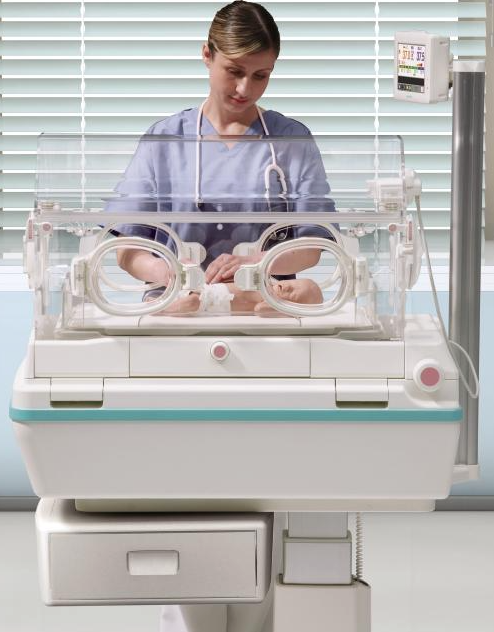
\includegraphics[width=.4\textwidth]{images/isolette.png}
\end{center}
\caption{Isolette}
\label{fig:isolette}
\end{figure}


Many babies have dies due to faulty incubators. There is thus a standard that manufacturers must satisfy. Modern incubators are equipped with alarms for air temperature, skin temperature, oxygen concentration and humidity. The alarms are both visual such as red warning lamps, and audio such as beep signals. Once measured measured values exceed permitted limits as well as when faults occur in sensors. For one such incident leading to death see ``Medical Devices: Use and Safety" shown in Fig.~\ref{fig:incubator}. 

\begin{figure}[!htb]
\begin{center}
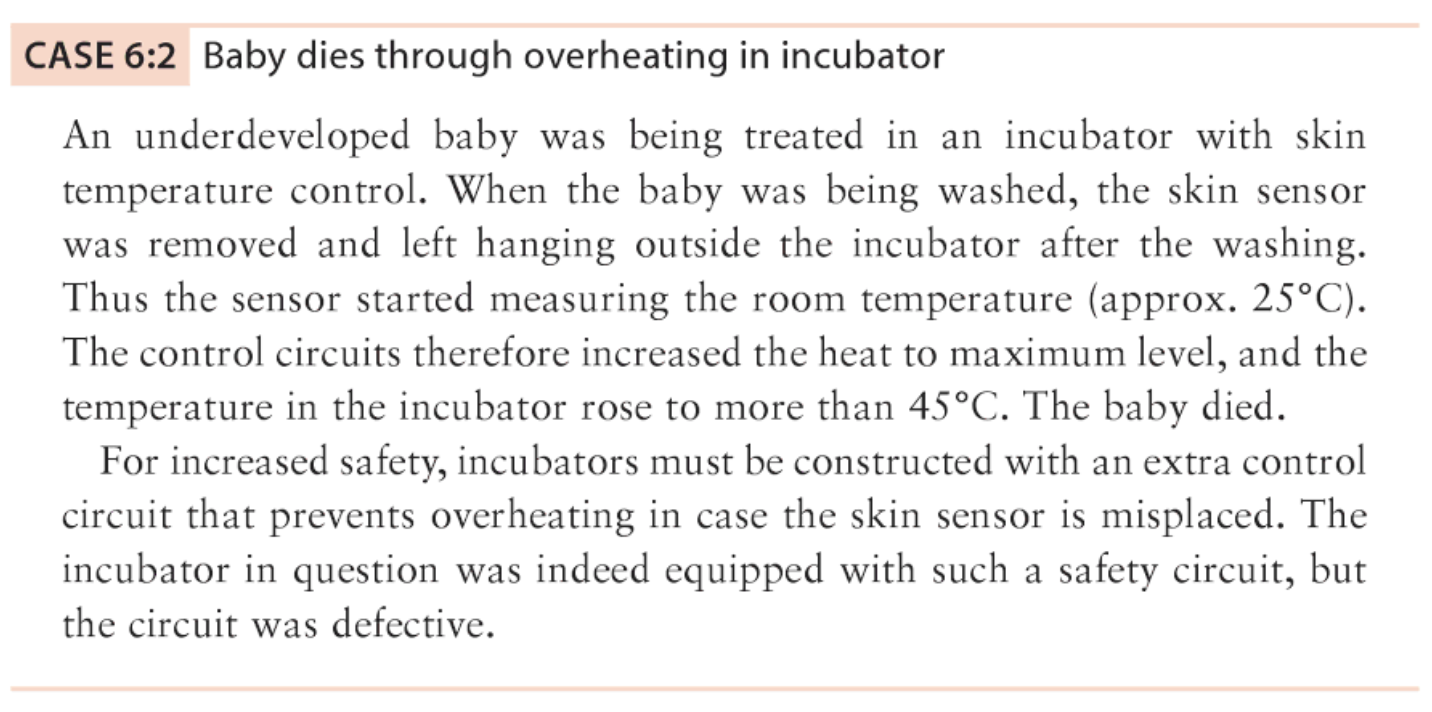
\includegraphics[width=.9\textwidth]{images/incubator.png}
\end{center}
\caption{Incubator Safety Problems \cite[p98]{JM2007}}
\label{fig:incubator}
\end{figure}

\section{Goals}

The high-level goals (G) of the system are:

\begin{mylist}
\item G1---The Infant should be kept at a safe and comfortable temperature.

\item G2---The Nurse should be warned if the Infant becomes too hot or too cold.

\item G3---The cost of manufacturing the computer controller for the thermostat should be as low as possible.
\end{mylist}


\newpage
\section{Context Diagram}

\begin{figure}[!htb]
\begin{center}
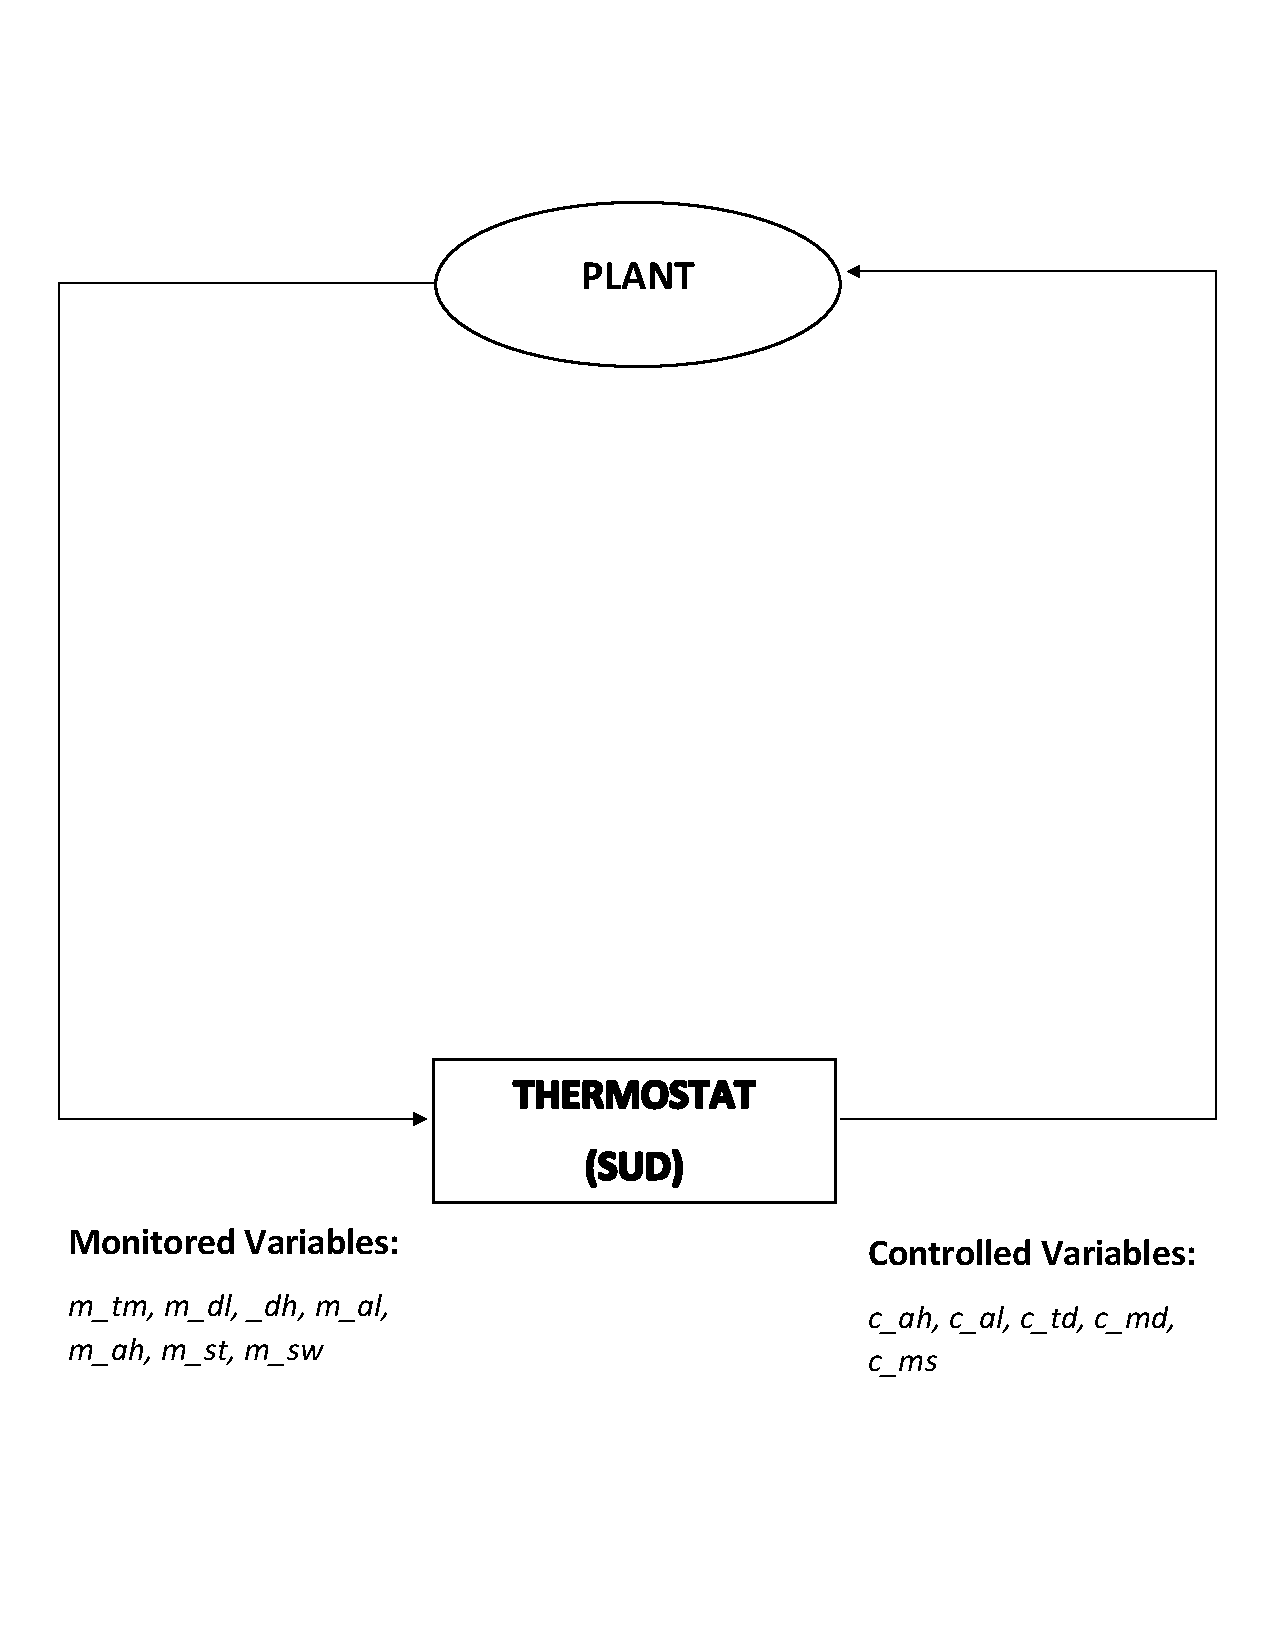
\includegraphics[width=.8\textwidth]{images/context-diagram.pdf}
\end{center}
\caption{Context diagram for the SUD}
\label{fig:context}
\end{figure}



\newpage
\section{Monitored Variables}

The monitored variables are a subset of those described in \cite{REMH}.\footnote{With some change of nomenclature. Monitored variables have an ``m'' prefix.} There is a single status variable \mv{st} that is \emph{invalid} whenever any one of the operator inputs or temperature sensor are in a failed state. Otherwise types and ranges are as in \cite{REMH}.

% Please add the following required packages to your document preamble:
% \usepackage[table,xcdraw]{xcolor}
% If you use beamer only pass "xcolor=table" option, i.e. \documentclass[xcolor=table]{beamer}
\begin{table}[h]
\begin{tabular}{|l|l|l|l|l|}
\hline
\cellcolor[HTML]{EFEFEF}Name & \cellcolor[HTML]{EFEFEF}Type & Range              & \cellcolor[HTML]{EFEFEF}Units & \cellcolor[HTML]{EFEFEF}Physical Interpretation                                       \\ \hline
\mv{tm}                      & $\Rl$                        &   $68 \upto 105$              &     $\degree{F}$                           & \begin{tabular}[c]{@{}l@{}}actual temperature of Isolette \\ air temperature from sensor\end{tabular} \\ \hline
\mv{dl}                      & $\intg$                      & $97 \upto 99$      & $\degree{F}$                   & \begin{tabular}[c]{@{}l@{}}desired lower temperature\\ set by operator\end{tabular}   \\ \hline
\mv{dh}                      & $\intg$                      &     $98 \upto 100$                            &    $\degree{F}$              & \begin{tabular}[c]{@{}l@{}}desired higher temperature\\ set by operator\end{tabular}  \\ \hline
\mv{al}                      & $\intg$                      &     $93 \upto 98$                            &    $\degree{F}$              & \begin{tabular}[c]{@{}l@{}}lower alarm temperature\\ set by operator\end{tabular}     \\ \hline
\mv{ah}                      & $\intg$                      &     $99 \upto 103$                         &   $\degree{F}$               & \begin{tabular}[c]{@{}l@{}}higher alarm temperature \\ set by operator\end{tabular}   \\ \hline
\mv{st}                      & Enumerated                   & \{valid, invalid\} &                               & \begin{tabular}[c]{@{}l@{}}status of sensor and \\ operator settings\end{tabular}     \\ \hline
\mv{sw}                      & Enumerated                   & \{on, off\}        &                               & switch set by operator                                                                \\ \hline
\end{tabular}
\caption{Monitored Variables}
\label{table:monitored}
\end{table}


\newpage
\section{Controlled Variables}

The controlled variables are a subset of those described in \cite{REMH}.\footnote{With some change of nomenclature. Controlled variables have a ``c'' prefix.} In addition, there is a mode display \cv{md} and a message display \cv{ms}.\footnote{The mode ``off'' is added to that of Fig.~A-4 in \cite{REMH}, and the mode transitions have been changed.}

% Please add the following required packages to your document preamble:
% \usepackage[table,xcdraw]{xcolor}
% If you use beamer only pass "xcolor=table" option, i.e. \documentclass[xcolor=table]{beamer}
\begin{table}[h]
\begin{tabular}{|l|l|l|l|l|}
\hline
\cellcolor[HTML]{EFEFEF}Name & \cellcolor[HTML]{EFEFEF}Type & Range                                                                    & \cellcolor[HTML]{EFEFEF}Units & \cellcolor[HTML]{EFEFEF}Physical Interpretation                                                         \\ \hline
\cv{hc}                      & Enumerated                   & \{on, off\}                                                              &                               & \begin{tabular}[c]{@{}l@{}}heat control: command to\\ turn heat source on or off\end{tabular}           \\ \hline
\cv{td}                      & $\intg$                      & $\{0\} \bunion \{68 \upto 105\}$                                         & $\degree{F}$                  & \begin{tabular}[c]{@{}l@{}}displayed temperature of Isolette\\ (zero when Isolette is off)\end{tabular} \\ \hline
\cv{al}                      & Enumerated                   & \{off, on\}                                                              &                               & sound alarm to call nurse                                                                               \\ \hline
\cv{md}                      & Enumerated                   & \begin{tabular}[c]{@{}l@{}}\{off, init, \\ normal, failed\}\end{tabular} &                               & \begin{tabular}[c]{@{}l@{}}mode of Isolette operation\\ (failed if $\mv{st} = invalid$)\end{tabular}    \\ \hline
\cv{ms}                      & Enumerated                   &                               \begin{tabular}[c]{@{}l@{}}\{ok, too\_hot\_alarm, \\ too\_cool\_alarm, warming\_up, \\ cooling\_down, system\_error\}\end{tabular}                 & & messages to display to nurse                                                                            \\ \hline
\end{tabular}
\caption {Controlled Variables}
\label{tbl:cv}
\end{table}

\newpage
\section{Mode Diagram}

\begin{figure}[!htb]
\begin{center}
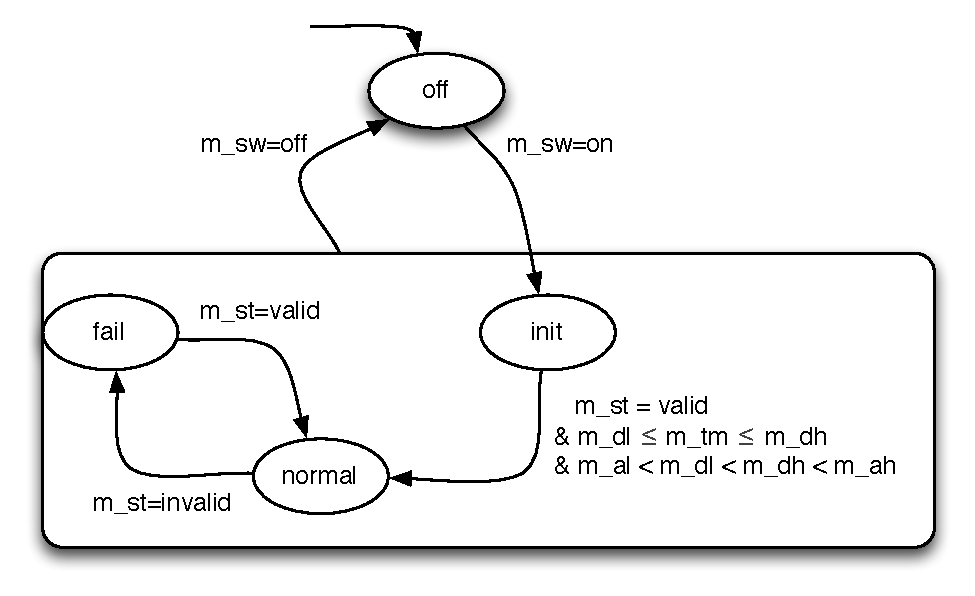
\includegraphics{images/mode-statechart.pdf}
\end{center}
\caption{Mode diagram for the states}
\label{fig:mode}
\end{figure}

\smallskip
\noindent \textbf{Rationale}: A mode diagram denotes the possible states the system can be in. They are \emph{abstract} variables whose output are visible to the client, in this case the nurse. In a particular state, the \emph{guard} condition has to be satisfied in order for the mode to change.


%% Deactivate this to place your own work
%% !TEX root = ../sel-report.tex
\section{What is a good requirement?}

\begin{mdframed}[outerlinewidth=0.5,roundcorner=5pt]
A requirement is a separately verifiable contractual statement
stating a need of the customer
\end{mdframed}

\begin{itemize}

\item The customer has certain needs and goals. However, those needs are likely to be vague or incomplete. If you build an actual product, it is hard to see how you (or your customer) would check that the product you built satisfies the customer's needs. What is needed is a \textbf{precise requirements document}.

\item A precise requirements document describes everything necessary to produce a safe and correct system---one that fulfills the needs of the customer---nothing more. 

\item The requirements document must provide the software developer with \textbf{all} the information needed for the system to be built.

\item At the same time the specification must not over-constrain developers by venturing into design and implementation detail.

\item The requirements document thus specifies \emph{what} the system will do---not \emph{how} the system will do it!

\end{itemize}

\section{System Under Description}

Some stuff. Here is a png figure (see folder ``pics'')

\begin{figure}[htb]
\includegraphics[width=.4\textwidth]{pics/sud.png}
\includegraphics[width=.4\textwidth]{pics/sud.pdf}
\caption{PDF (right) displays better than jpeg or png (right)}
\label{fig:1}
\end{figure}

See Fig.~\ref{fig:1} for how to put an image in a figure environment. The ``htb'' says put the figure first here, then top of the page, then bottom, depending on layout algorithm. 

\section{R-descriptions and E-descriptions}
\reqm{ENV}
{Although it is physically possible for the trip and keypad commands to occur at the same time, the system is hardwired to respond sequentially (i.e. there is an arbitrary choice which one is dealt with first). Thus all signals arrive sequentially.}
{Refer to where your mathematical model uses this}
\label{E1}


\reqm{REQ}
{If the system is armed then a trip signal from the motion detector shall result in the siren being sounded.\\}
{Refer to mathematical model}
\label{R2}

\subsection{Subsection heading}

Other stuff with inline maths $p \limp q$ and 

\begin{equation}\label{eqn:1}
p \land q \lor r \limp z
\end{equation}

In (\ref{eqn:1}), we see how to write a formula.

Here is a verbatim environment with smaller text:

\begin{code}
=========================================
Use Case 1: uc1.txt: adding product types
=========================================
  report:      ok
  id:          0
  products:   
  stock:       
  orders:      
  carts:       
  order_state: 
->add_type("nuts")
  report:      ok
  id:          0
  products:    nuts
  ..
\end{code}

Here is some formatted PVS
\begin{pvs}
gate: THEORY
BEGIN
  p, q, r: bool
  not_gate(x: bool): bool = NOT x
  and_gate(x:bool, y:bool): bool = x AND y
  or_gate(x:bool, y:bool): bool = x OR y
  check1: CONJECTURE and_gate(p, not_gate(q)) => (p AND NOT q)
  check2: CONJECTURE and_gate(p, not_gate(q)) =  (p AND NOT q)

  circuit_implementation(x:bool, y:bool): bool = 
    and_gate(
              (or_gate(  and_gate(x, not_gate(y))
                       , and_gate(x,y))
             , y))

   and_conjecture: CONJECTURE
     and_gate(p,q) = circuit_implementation(p,q)

   or_conjecture:  CONJECTURE
     or_gate(p,q)  = circuit_implementation(p,q)
END gate
\end{pvs}

\begin{textbox}
Some text
\end{textbox}

\subsection{Signum Function}
Let's start with a simple example. In mathematics, the sign function or signum  (from \emph{signum}, Latin for ``sign") function $sgn(x)$ --- is a mathematical function that extracts the sign of a real number. In mathematical expressions the sign 

\begin{figure}[ht]
\begin{mdframed}[outerlinewidth=0.5,roundcorner=5pt]
\begin{minipage}{.4\textwidth}
\[sgn(x:\Rl) =
\begin{cases}
-1, &\text{if $x < 0$;}\\
0, &\text{if $x=0$;}\\
1, &\text{if $x >0$.}
\end{cases}\]
\end{minipage}
\qquad\qquad\qquad
\begin{minipage}{.5\textwidth}
\begin{tabular}{|l|l|}
\hline
        & $sgn(x)$ \\ \hline
$x < 0$ & -1     \\ \hline
$x = 0$ & 0      \\ \hline
$x > 0$ & 1      \\ \hline
\end{tabular}
\end{minipage}
\end{mdframed}
\caption{\small (a) Standard mathematical definition of $sgn(x)$. (b) Function table definition}
\end{figure}

The normal mathematical definition and the table layout are identical in meaning. However, the table layout is easier on the reader. Note that both description methods are \textbf{complete} and \textbf{disjoint}. 

\subsection*{Completeness}
The description of $sgn$ is complete because the function is defined for all possible inputs $x\in \Rl$. 

\subsection*{Disjointness}
The description is disjoint because each row in the table describes a case that is independent of the other rows --- hence avoiding inconsistencies 
--- where the same condition triggers different (and possibly contradictory) behaviours. 

For example, in a computer controlling a robot, we would not want the press of a \emph{move} button to signall to a robot to move right and move left at the same time.

The listing below shows how to describe the function in PVS.\footnote{%
See \url{https://wiki.eecs.yorku.ca/project/sel-students/p:tutorials:pvs:start}.}

 \section{Bibliography}
 
 See this \cite{Lamsweerde09}, this\ cite{GS93} and this \cite{Spivey92}. Run bibtex and then latex three times. 
\bibliographystyle{plain}
\bibliography{ref}

\newpage
\section{R-Descriptions}

The following are the R-descriptions for the System Under Description.

\rdescription
{The \emph{controller} shall operate in one of four modes: \emph{off}, \emph{init}, \emph{normal} and \emph{fail}.\\}
{See statechart in Fig.~\ref{fig:mode}.}
\label{R1}

\smallskip
\noindent \textbf{Rationale}: The Isolette can show four statuses to the Nurse.
\begin{mylist}
\item \emph{off} mode indicates that the Isolette is switched off. If the Isolette gets switched on, move to the \emph{init} state.
\item \emph{init} mode indicates that the Isolette has just been switched on and the temperature sensor is still not in the desired range. If the input from the nurse is valid and the temperatures are in their desired ranges then move to the \emph{normal} state.
\item \emph{normal} mode indicates everything is under control (i.e all inputs are correct and the sensors are working fine). If something goes wrong, then move on to the \emph{fail} state.
\item \emph{fail} mode indicates something went wrong and sound an alarm. The nurse can either then turn the Isolette off to go to the \emph{off} state or fix the input temperature ranges to go back to the \emph{normal} state.
\end{mylist} 

\rdescription
{In the \emph{normal} mode, the temperature controller shall maintain current temperature inside the Isolette within a set temperature range (the \emph{desired} range).\\}
{The \emph{desired} temperature range is $\mv{dl} \upto \mv{dh}$. If the current temperature \mv{tm} is outside this range, the controller shall turn the heater on or off via the controlled variable \mv{hc} to maintain the desired state.\smallskip}
\label{R2}

\smallskip
\noindent \textbf{Rationale}: The \emph{desired temperature range} will be set by the nurse to the desired range based on the infant's weight and health. The controller shall maintain the current temperature within this range under normal operation.

The following relevant hazard was identified through the safety assessment process:
\begin{mylist}
\item \textbf{H1}: Prolonged exposure of Infant to unsafe heat or cold;
\item \emph{Classification}: catastrophic;
\item \emph{Probability}: $<10^{-9}$ per hour of operation.
\end{mylist}

\noindent To ensure that probability of hazard H1 is $10^{-9}$ per hour of operation, the following derived safety requirement shall apply to the Isolette controller: 

\rdescription
{In \emph{normal} mode, the controller shall activate an alarm whenever 

\begin{mylist}
\item the current temperature falls outside the \emph{alarm} temperature range (either through temperature fluctuation or a change in the alarm range by an operator), or
\item a failure is signalled in any of the input devices (temperature sensor and operator settings).
\end{mylist}~}
{The alarm temperature range is $\mv{al}\upto\mv{ah}$.

Monitored variable \mv{st} 
in Table~\ref{table:monitored} 
shows ``invalid'' when any of the input signals fail.}
\label{R3}

\smallskip
\noindent \textbf{Rationale}: The alarm needs to go off to alert the nurse during critical situations. Most importantly, in the \emph{normal} mode since that is when the child is first put into the Isolette. It must be ensured that the Isolette is capable of handling the child and in any case when it cannot, an alarm must go off to notify the nurse.

\rdescription
{Once the alarm is activated, it becomes deactivated in one of two ways:
\begin{mylist}
\item The nurse turns off the Isolette;
\item The alarm has lasted for 10 seconds, and after 10 seconds or more the alarm conditions are removed.
\end{mylist}~\\}
{The Isolette can be switched off by setting \emph{m\_sw} to off. The alarm condition can be removed when the alarm \emph{c\_hc} has been activated for more than 10 seconds. Refer to Table  ~\ref{tbl:cv} and ~\ref{tbl:al}.}
\label{R4}

\smallskip
\noindent \textbf{Rationale}: The Alarm Temperature Range will be set by the Nurse based on the Infant’s weight and health. Once the alarm is activated (i.e the temperature falls beyond the range), the Infant should be removed from the Isolette and the Isolette should be turned off. If the nurse fails to accomplish that within 10 seconds, the alarm gets deactivated with the infant inside.

\rdescription
{If mode is \emph{normal} and the value of the Current Temperature is greater than or equal to the Lower Alarm Ttemperature +0.5° and less than or equal to the Upper Alarm Temperature -0.5°, the alarm shall be set to \emph{off}.}
{When the current temperature is between +/-0.5 of the alarm temperature range, $m\_al+0.5 <= m\_tm <= m\_ah - 0.5$ then \emph{c\_al} should be set to off. Refer to Table ~\ref{tbl:cv} and ~\ref{tbl:al}.}
\label{R5}

\smallskip
\noindent \textbf{Rationale}: The alarm should be turned off at the same moment that the Displayed Temperature shows a value greater than the Lower Alarm Temperature and less than the Upper Alarm Temperature.

\rdescription
{The Thermostat shall set the value of the Heat Control depending on the Current Temperature.}
{The heat control of the Isolette is the control variable \emph{c\_hc}. Refer to Table ~\ref{tbl:cv} and ~\ref{tbl:hc}.}
\label{R6}

\smallskip
\noindent \textbf{Rationale}: The controlled variable \emph{c\_hc} is used by the thermostat to turn the Heat Control on and off to maintain the Current Temperature in the Isolette within the Desired Temperature Range, i.e within \emph{m\_dl} and \emph{m\_dh}. If the Current Temperature is below the Desired Low Temperature, the heat control should be set on. If the Current Temperature is above the Desired High Temperature, the heat control should be set off.

\rdescription
{In the \emph{init} and \emph{normal} modes, the displayed temperature shall be set to the value of the current temperature rounded to the nearest integer.}
{The displayed temperature of the Isolette is the control variable \emph{c\_td}. Refer to Table ~\ref{tbl:cv} and ~\ref{tbl:td}.} %~\ref{}}
\label{R7}

\smallskip
\noindent \textbf{Rationale}: The controlled variable \emph{c\_td} is used by the thermostat to show the Current Temperature of the Isolette. The Displayed Temperature is calculated using the mathematical floor function of the Current Temperature to avoid showing invalid temperatures to the nurse.

%%%%%%%%%%%%%%%%%%%%%%%%%%%%%%
\newpage
\section{E-descriptions}

The following are the environmental assumption made on the Isolette System:

\edescription
{The current temperature received from the sensor is a a real number in the range $68.0$ to $105.0 \degree{F}$.\\}
{The monitored variable \emph{m\_tm} in Table ~\ref{table:monitored} specifies the range, type and unit for the Current Temperature received from the sensor.}
\label{E1}

\smallskip
\noindent \textbf{Rationale}: This is the specified range of operation of the Isolette. The lower end of this range is useful for monitoring an Isolette that is warming to the Desired Temperature Range. The upper end is set to be greater than the Higher Alarm Temperature.

\edescription
{The desired and alarm temperatures received from the operator are all in increments of $1 \degree{F}$.\\}
{The monitored variables \emph{m\_tm}, \emph{m\_dl}, \emph{m\_dh}, \emph{m\_al} and \emph{m\_ah} set in an increment of $1 \degree{F}$. Refer to Table ~\ref{table:monitored} to see details about the monitored inputs.}
\label{E2}

\smallskip
\noindent \textbf{Rationale}: Marketing studies have shown that customers prefer to set temperatures in 1 degree increments. A resolution 1°F is sufficient to be consistent with the functionality and performance for the Isolette.

\edescription
{The Lower Alarm Temperature will always be $ >= 93\degree{F}$.\\}
{The monitored variables \emph{m\_al} denotes the Lower Alarm Temperature. Table ~\ref{table:monitored} specifies the range, type and unit for the Lower Alarm Temperature set by the Nurse.}
\label{E3}

\smallskip
\noindent \textbf{Rationale}: Exposure to temperatures less than $93\degree{F}$ will result in hypothermia, which can lead to death within a few minutes for severely ill pre-term infants.

\edescription
{The Higher Alarm Temperature will always be $ <= 103\degree{F}$.\\}
{The monitored variables \emph{m\_ah} denotes the Higher Alarm Temperature. Table ~\ref{table:monitored} specifies the range, type and unit for the Higher Alarm Temperature set by the Nurse.}
\label{E4}

\smallskip
\noindent \textbf{Rationale}: Exposure to temperatures greater than $103\degree{F}$ will result in hyperthermia, which can lead to cardiac arrhythmias and febrile seizures within a few minutes.

\edescription
{The Lower Desired Temperature will always be $ >= 97\degree{F}$.\\}
{The monitored variables \emph{m\_dh} denotes the Lower Desired Temperature. Table ~\ref{table:monitored} specifies the range, type and unit for the Lower Desired Temperature set by the Nurse.}
\label{E5}

\smallskip
\noindent \textbf{Rationale}: Exposing the Infant to temperatures lower than $97\degree{F}$ may result in excessive heat loss and drop in heart rate secondary to metabolic acidosis.


%%%%%%%%%%%%%%%%
\newpage
\section{Abstract variables needed for the Function Table}

No abstract variables were used for the function tables.

\newpage
%%%%%%%%%%%%%%%%%%%%%%%%%%%%
\section{Function Tables}

Below are the function tables for each of the controlled variables:\\

\subsection{Function Table for Mode Control: \cv{md}}

\begin{table}[h]
\centering
\begin{tabular}{| c | c | c | c| c |}
	\cline{5-5}
	\multicolumn{4}{ c| }{ }& $c\_md(i)$  \\\hline
	\multicolumn{4}{ |c| }{ $ i= 0$}& {\multirow{2}{*}{$off$}} \\ \cline{1-4}

    {\multirow{9}{*}{$i>0$}}  & \multicolumn{3}{ c| }{ $m\_sw(i) = off$} & \\ \cline{2-5}
          & {\multirow{7}{*}{$\neg(m\_sw(i) = off)$ }}&  \multicolumn{2}{ c| }{ $c\_md(i - 1) = off$ }   &  $init $\\ \cline{3-5}
          & &  {\multirow{2}{*}{$c\_md(i - 1) = init$ }}                & $ S_{1}$ & $normal$ \\ \cline{4-5}
	    & &                                                                         & $ \neg S_{1}$ &  $c\_md(i-1)$   \\ \cline{3-5}
	    & &   {\multirow{2}{*}{$c\_md(i - 1) = normal$ }}       & $m\_st(i)=invalid$ & $fail$ \\ \cline{4-5}
	    & &                                                                          & $m\_st(i)=valid$ & {\multirow{2}{*}{$c\_md(i-1)$}}  \\ \cline{3-4}
         & &  {\multirow{2}{*}{$c\_md(i - 1) = fail$ }}             & $m\_st(i)=invalid$ &   \\ \cline{4-5}
	    & &               & $m\_st(i)=valid$  & $normal$  \\ \hline
\end{tabular}
\caption {Function Table for Mode Control}
\label{tbl:cmd}
\end{table}

\begin{table}[h]
\subparagraph{}
\centering
\begin{tabular}{| c | l | l |}
	\hline
     {\multirow{3}{*}{$S_{1}$ }} & $m\_st(i)=valid \land $  & This is the condition \\ 
	                                          & $m\_dl(i)\leq m\_tm(i)\leq m\_dh(i) \land $  & to be met for system to go \\ 
	                                          & $m\_al(i) < m\_dl(i) < m\_dh(i) < m\_ah(i) $  & from $init$ to $normal$\\ \hline
\end{tabular} 
\caption {Definition of $S_1$}
\label{tbl:cmd1}
\end{table}


\newpage
\subsection{Function Table for Heat Control: \cv{hc}}

\begin{table}[h]
\centering
\begin{tabular}{| c | c | c | p{4.5cm} | c |}
	\cline{5-5}
	\multicolumn{4}{ c| }{ }& $c\_hc(i)$  \\\hline
	\multicolumn{4}{ |c| }{ $ i= 0$}& {\multirow{2}{*}{$off$}} \\ \cline{1-4}

    {\multirow{5}{*}{$i>0$}}  & \multicolumn{3}{ c| }{ $m\_sw(i) = off$} & \\ \cline{2-5}
          & {\multirow{4}{*}{$\neg(m\_sw(i) = off)$ }}&  \multicolumn{2}{ c| }{ $ \neg(m\_dl(i) < m\_dh(i))$ }   &  $c\_hc(i-1) $\\ \cline{3-5}
          & &  {\multirow{3}{*}{$ m\_dl(i) < m\_dh(i)$ }}                & $ m\_tm(i) < m\_dl(i)$ & $on$ \\ \cline{4-5}
	    & &                                                                                        & $ m\_dl(i) <= m\_tm(i) \land m\_tm(i) <= m\_dh(i) $ &  $c\_hc(i - 1)$   \\ \cline{4-5}
	    & &                                                                                        & $ m\_tm(i) > m\_dh(i)$ &  $off$   \\ \hline
\end{tabular}
\caption {Function Table for Heat Control}
\label{tbl:hc}
\end{table}


\newpage
\subsection{Function Table for Tempearature Display Control: \cv{td}}
\begin{table}[h]
\centering
\begin{tabular}{| c | c | c |}
	\cline{3-3}
	\multicolumn{2}{ c| }{ }& $c\_td(i)$  \\\hline
	\multicolumn{2}{ |c| }{ $ i= 0$} & {\multirow{2}{*}{$0$}} \\ \cline{1-2}
    {\multirow{2}{*}{$i>0$}}  & $c\_md(i - 1) = off \lor c\_md(i - 1) = fail $ & \\ \cline{2-3}
           & $c\_md(i - 1) = init \lor c\_md(i - 1) = normal$ & $ floor(m\_tm(i) + 0.5)$  \\ \hline
     
\end{tabular}
\caption {Function Table for Temperature Display Control}
\label{tbl:td}
\end{table}

\newpage
\subsection{Function Table for Message Display Control: \cv{ms}}
\begin{table}[h]
\centering
\begin{tabular}{| c | c | }
	\cline{2-2}
	\multicolumn{1}{ c| }{ }& $c\_ms(i)$ \\ \hline
	$m\_st(i) = invalid $      &  $system\_error$ \\ \hline
	$m\_tm(i) > m\_ah(i) $  &  $too\_hot\_alarm$  \\ \hline
	$m\_tm(i) < m\_al(i) $   &   $too\_cool\_alarm$ \\ \hline
	$m\_al(i) < m\_tm(i) < m\_dl(i) $ & $warming\_up$ \\ \hline
	$m\_dh(i) < m\_tm(i) < m\_ah(i) $ & $cooling\_down$ \\ \hline
     $ELSE $ & $ok$ \\ \hline
\end{tabular}
\caption {Function Table for Message Display Control}
\label{tbl:ms}
\end{table}

\newpage
\subsection{Function Table for Alarm Control: \cv{al}}
\begin{table}[h]
\centering
\begin{tabular}{| c | c | c | c | c | c | c | c |}
	\cline {8-8}

	\multicolumn{7}{ c| }{ }  & $c\_al(i)$ \\ \hline

	\multicolumn{7}{|c| }{$i=0$ } & {\multirow{2}{*}{$off$}} \\ \cline{1-7}
	{\multirow{7}{*}{$i>0$}} & \multicolumn{6}{ c| }{$S_2$} &  \\ \cline{2-8}
	  & {\multirow{6}{*}{$\neg S_2$}} & \multicolumn{5}{ c| }{ $S_3$} & $c\_al(i - 1)$ \\ \cline{3-8}
	  &   &  {\multirow{5}{*}{$\neg S_3$}} & \multicolumn{4}{ c| }{$S_4$} &  $on$ \\ \cline{4-8}
	  &   &   & {\multirow{4}{*}{$\neg S_4$}} & \multicolumn{3}{ c| }{$c\_al(i - 1) = off$} & $c\_al(i - 1)$ \\ \cline{5-8}
	  &   &   &   & {\multirow{3}{*}{$c\_al(i - 1) = on$}} & \multicolumn{2}{ c| }{$S_5$} & {\multirow{2}{*}{$off$}} \\ \cline{6-7}
	  &   &   &   &   & {\multirow{2}{*}{$\neg S_5$}} & $m\_sw(i) = off$ & \\ \cline{7-8}
	  &   &   &   &   &   & $m\_sw(i) = on$ & $on$  \\ \hline

\end{tabular}
\caption {Function Table for Alarm Control}
\label{tbl:al}
\end{table}

\begin{table}[h]
\subparagraph{}
\centering
\begin{tabular}{| c | l | l |}
	\hline
	{\multirow{2}{*}{$S_2$ }}  & $c\_md(i - 1) = off \lor c\_md(i - 1) = init$  &  Mode is $off$ or $init$.  \\
								  & &Else it is in $normal$ or $fail$ mode.  \\  \hline
     {\multirow{2}{*}{$S_3$ }} & $(m\_al(i) <= m\_tm(i) \land m\_tm(i) < m\_al(i) + 0.5) \lor$  &  This is the  \\ 
	                                        & $ (m\_ah(i) - 0.5 <= m\_tm(i) \land m\_tm(i) <= m\_ah(i))$  &  Hysteresis Region. \\ \hline

	{\multirow{2}{*}{$S_4$ }}  & $ m\_tm(i) > m\_ah(i)  \lor m\_tm(i) < m\_al(i) \lor$  &  Conditions for  \\ 
	                                        & $ m\_st(i) = invalid$  &when the alarm is on.  \\ \hline

	{\multirow{2}{*}{$S_5$ }}  & $held\_for(alarm, 10)(i - 1)$ &  Checks if alarm was  \\ 
	                                        & & on for at least 10 seconds.  \\ \hline
\end{tabular} 
\caption {Definitions for $S_2$, $S_3$, $S_4$ and $S_5$}
\label{tbl:al1}
\end{table}
%% \hl{Function table goes here on this page. Other function tables each on their own page}

%%%%%%%%%%%%%%%%%%%%%%%%%%%%
\newpage
\section{Validation}
\hl{To be Done.} 
Proof of completeness and disjointness and validation of the requirements using PVS.

Include the PVS sources in the appendix to this document but summarize the proofs here.

%%%%%%%%%%%
\newpage
\section{Use Cases}

The following use case is defined informally and then formally using logic in PVS:\\


a) \textbf{Informal}: Assume the Isolette is switched on and an infant has already been placed in the incubator. The Isolette is in the normal mode and certainly the current temperature drops below the lower alarm temperature without any other fault in the sensors. Then the alarm should become \textbf{activated} and the message displayed to the the nurse should indicate the the Isolette is too cool.\\

b) \textbf{Formal}: Below is the PVS conjecture for the above use case:
\begin{pvs}
  usecase4: CONJECTURE
        c_md(2) = normal 
        AND m_sw(3) = on 
        AND m_tm(3) = 90
     	AND m_al(3) = 93 
     	AND m_ah(3) = 103 
     	AND NOT (m_st(3) = invalid)
     	AND alarm_ft(3) 
     	AND message_ft(3) 
     	AND mode_ft(3)
     	IMPLIES 
     	c_al(3) = on 
     	AND c_ms(3) = too_cool_alarm 
     	AND c_md(3) = c_md(2) 	
\end{pvs}

\smallskip
\noindent Refer to section ~\ref{auc} for additional use cases.


%%%%%%%%%%%%%%%%%
\newpage
\section{Acceptance Tests}

In this section, the use cases have to be converted into precise acceptance tests (using the function table to describe pre/post conditions) to be run when the design and implementation are complete. \hl{Describe one acceptance test}

%%%%%%%%%%%%%%%%%
\newpage
\section{Traceability}

Matrix to show which acceptance tests passed, and which R-descriptions they checked. No need to do this for this assignment. 


\section{Glossary}

The definition of important terms is placed in this section. You are not required to complete this.
%%%%%%%%%%%%%%%%%%%%%%%%%%%%%%%%%%%%%
\bibliographystyle{plain}
\bibliography{ref}

\newpage
\appendix

\section{PVS Time Theory for held-for operator}

Below is the PVS Theory for the using the \emph{held-for} operator:\\

\begin{pvs}
Time[delta: posreal]: THEORY
 BEGIN

  DTIME: TYPE = nat

  init(i: DTIME): bool = i = 0

  RTIME: TYPE = {t: nnreal | (EXISTS (i: DTIME): t = i * delta)}

  TIME: TYPE = nnreal

  POS_DTIME: TYPE = posnat

  r2d(t: RTIME): DTIME = t / delta

  d2r(i: DTIME): RTIME = i * delta

  DURATION: TYPE = nnreal

  held_for(p: pred[DTIME], d: DURATION)(i: DTIME): bool =
      (FORALL (j: int):
         i - (d / delta) <= j AND j <= i IMPLIES 0 <= j AND p(j))
 END Time	
\end{pvs}

\newpage
\section{PVS Isolette Theory}

Below is the PVS Theory for the Isolette Specification:\\

\begin{pvs}
% Isolette System Specification

Isolette[delta: posreal]: THEORY
 BEGIN
  % importing Time specification
  IMPORTING Time[delta]

  % variable
  i: VAR DTIME

  % types
  CURRENT_TEMPERATURE: TYPE = {n: real | n >= 68.0 AND n <= 105.0}
        CONTAINING 68.0

  DESIRED_LOW_TEMP: TYPE = {n: integer | n >= 97 AND n <= 99} 
  		CONTAINING 97

  DESIRED_HIGH_TEMP: TYPE = {n: integer | n >= 98 AND n <= 100} 
  		CONTAINING 98

  ALARM_LOW_TEMP: TYPE = {n: integer | n >= 93 AND n <= 98} 
  		CONTAINING 94

  ALARM_HIGH_TEMP: TYPE = {n: integer | n >= 99 AND n <= 103} 
  		CONTAINING 100

  STATUS: TYPE = {valid, invalid}

  SWITCH: TYPE = {on, off}

  HEAT_CONTROL: TYPE = {on, off}

  DISPLAYED_TEMPERATURE: TYPE =
        {n: integer | n = 0 OR n >= 68 AND n <= 105} CONTAINING 68
\end{pvs}
\newpage
\begin{pvs}
  MESSAGES: TYPE =
  {ok, cooling_down, warming_up, too_cool_alarm, too_hot_alarm,
   system_error}

  ALARM: TYPE = {off, on}

  MODES: TYPE = {off, init, normal, fail}

  % monitored variables
  m_tm: [DTIME -> CURRENT_TEMPERATURE]

  m_dl: [DTIME -> DESIRED_LOW_TEMP]

  m_dh: [DTIME -> DESIRED_HIGH_TEMP]

  m_al: [DTIME -> ALARM_LOW_TEMP]

  m_ah: [DTIME -> ALARM_HIGH_TEMP]

  m_st: [DTIME -> STATUS]

  m_sw: [DTIME -> SWITCH]

  % controlled variables
  c_hc: [DTIME -> HEAT_CONTROL]

  c_td: [DTIME -> DISPLAYED_TEMPERATURE]

  c_ms: [DTIME -> MESSAGES]

  c_al: [DTIME -> ALARM]

  c_md: [DTIME -> MODES]

  alarm(i: DTIME): bool = c_al(i) = on
  \end{pvs}
  \newpage
  \begin{pvs}
  % FUNCTION TABLES %
  
  % mode function table: c_md
  mode_ft(i): bool =
      COND i = 0 -> c_md(i) = off,
           i > 0 ->
             COND m_sw(i) = off -> c_md(i) = off,
                  NOT (m_sw(i) = off) ->
                    COND c_md(i - 1) = off -> c_md(i) = init,
                         c_md(i - 1) = init ->
                           COND m_st(i) = valid
                                      AND m_dl(i) <= m_tm(i)
                                      AND m_tm(i) <= m_dh(i)
                                      AND m_al(i) < m_dl(i)
                                      AND m_dl(i) < m_dh(i)
                                      AND m_dh(i) < m_ah(i)
                            		  -> c_md(i) = normal,
                                NOT (m_st(i) = valid
                                      AND m_dl(i) <= m_tm(i)
                                      AND m_tm(i) <= m_dh(i)
                                      AND m_al(i) < m_dl(i)
                                      AND m_dl(i) < m_dh(i)
                                      AND m_dh(i) < m_ah(i))
                                  	  -> c_md(i) = c_md(i - 1)
                           ENDCOND,
                         c_md(i - 1) = normal ->
                           COND m_st(i) = invalid -> c_md(i) = fail,
                                NOT (m_st(i) = invalid) ->
                                  c_md(i) = c_md(i - 1)
                           ENDCOND,
                         c_md(i - 1) = fail ->
                           COND NOT (m_st(i) = invalid) ->
                                  c_md(i) = normal,
                                m_st(i) = invalid -> 
                                c_md(i) = c_md(i - 1)
                           ENDCOND
                    ENDCOND
             ENDCOND
      ENDCOND
  \end{pvs}
  \newpage
  \begin{pvs}
  % heat control function table: c_hc    
  heat_control_ft(i): bool =
      COND i = 0 -> c_hc(i) = off,
           i > 0 ->
             COND m_sw(i) = off -> c_hc(i) = off,
                  NOT (m_sw(i) = off) ->
                    COND m_dl(i) < m_dh(i) ->
                           COND m_tm(i) < m_dl(i) -> c_hc(i) = on,
                                m_dl(i) <= m_tm(i) 
                                AND m_tm(i) <= m_dh(i)
                                	-> c_hc(i) = c_hc(i - 1),
                                m_tm(i) > m_dh(i)
                                	-> c_hc(i) = off
                           ENDCOND,
                         NOT (m_dl(i) < m_dh(i)) 
                         	-> c_hc(i) = c_hc(i - 1)
                    ENDCOND
             ENDCOND
      ENDCOND

  % temperature display function table: c_td
  temperature_display_ft(i): bool =
      COND i = 0 -> c_td(i) = 0,
           i > 0 ->
             COND 
             	c_md(i - 1) = off OR c_md(i - 1) = fail 
             		-> c_td(i) = 0,
                c_md(i - 1) = init OR c_md(i - 1) = normal
                	-> c_td(i) = floor(m_tm(i) + 0.5)
             ENDCOND
      ENDCOND
  \end{pvs}
  \newpage
  \begin{pvs}
  % alarm control function table: c_al    
  alarm_ft(i): bool =
      COND i = 0 -> c_al(i) = off,
           i > 0 ->
           COND c_md(i - 1) = off OR c_md(i - 1) = init -> 
           	  c_al(i) = off,
                c_md(i - 1) = normal OR c_md(i - 1) = fail ->
                COND ((m_al(i) <= m_tm(i) 
                      AND m_tm(i) < m_al(i) + 0.5)
                      OR
                      (m_ah(i) - 0.5 <= m_tm(i) 
                      AND m_tm(i) <= m_ah(i))) ->
                      c_al(i) = c_al(i - 1),
                      NOT ((m_al(i) <= m_tm(i) 
                           AND m_tm(i) < m_al(i) + 0.5)
                           OR
                           (m_ah(i) - 0.5 <= m_tm(i) 
                           AND m_tm(i) <= m_ah(i))) ->
                           COND (m_tm(i) > m_ah(i) 
                                OR m_tm(i) < m_al(i) 
                                OR m_st(i) = invalid) -> 
                                c_al(i) = on,
                               	NOT (m_tm(i) > m_ah(i)
                                     OR
                                     m_tm(i) < m_al(i)
                                     OR
                                     m_st(i) = invalid) ->
                                     COND c_al(i - 1) = off -> 
                                     	  c_al(i) = c_al(i - 1),
                                          NOT (c_al(i - 1) = off) ->
                                          COND
                                          held_for(alarm, 10)(i - 1)
                                          -> c_al(i) = off,
                                          NOT
                                          (held_for(alarm, 10)
                                          (i - 1))
                                          ->
                                          COND m_sw(i) = off -> 
                                            c_al(i) = off,
                                       	    NOT (m_sw(i) = off) ->
                                            c_al(i) = on
                                          ENDCOND
                                       ENDCOND
                                  ENDCOND
                           ENDCOND
                    ENDCOND
             ENDCOND
      ENDCOND
      
  % displayed message functional table: c_ms
  message_ft(i): bool =
      IF m_st(i) = invalid THEN c_ms(i) = system_error
      ELSIF m_tm(i) > m_ah(i) THEN c_ms(i) = too_hot_alarm
      ELSIF m_tm(i) < m_al(i) THEN c_ms(i) = too_cool_alarm
      ELSIF m_al(i) < m_tm(i) < m_dl(i) THEN c_ms(i) = warming_up
      ELSIF m_dh(i) < m_tm(i) < m_ah(i) THEN c_ms(i) = cooling_down
      ELSE c_ms(i) = ok
      ENDIF
  
  % specification of all function tables
  specification(i): bool =
           mode_ft(i) AND heat_control_ft(i) 
           AND temperature_display_ft(i)
       	   AND alarm_ft(i) AND message_ft(i)

  % INVARIANTS %
  
  % inv1: All modes are in the set of { off, init, normal, fail }
  invariant1(i): bool =
      c_md(i) = off OR c_md(i) = init OR c_md(i) = normal 
      OR c_md(i) = fail

  % inv2: All messages are in the set of { system_error, 
  % too_hot_alarm, too_cool_alarm, warming_up, 
  % cooling_down, ok }
  invariant2(i): bool =
          c_ms(i) = system_error OR c_ms(i) = too_hot_alarm
       	  OR c_ms(i) = too_cool_alarm OR c_ms(i) = warming_up
          OR c_ms(i) = cooling_down OR c_ms(i) = ok
   
  % inv3: The heat control cannot be on and off at the same time     
  invariant3(i): bool = NOT (c_hc(i) = on AND c_hc(i) = off)
  \end{pvs}
  \newpage
  \begin{pvs}
  % inv4: The alarm cannot be on and off at the same time
  invariant4(i): bool = NOT (c_al(i) = on AND c_al(i) = off)

  % all the invariants
  invariant(i): bool =
      		invariant1(i) AND invariant2(i) AND invariant3(i) 
      		AND invariant4(i)

  % specficiation should satisfy the invariant
  spec_inv_holds: CONJECTURE
    		FORALL (i: DTIME): 
    		specification(i) 
    		IMPLIES 
    		invariant(i)

  % USECASES %
  
  % uc1: If the switch is on and the status is invalid 
  % then the message displayed should say "system_error"
  usecase1: CONJECTURE
    	m_sw(2) = on AND m_st(2) = invalid AND message_ft(2) 
    	IMPLIES
    	c_ms(2) = system_error

  % uc2: If the switch is on at time 1 and the current temperature 
  % is outside the temperature range at time 1 THEN 
  % the mode at time 0 is off and mode at time 1 is init
  usecase2: CONJECTURE
         m_sw(1) = on AND m_tm(1) = 74 AND m_al(1) = 97 
         AND m_ah(1) = 103 AND m_dl(1) = 98 
         AND m_dh(1) = 100 AND m_st(1) = valid AND mode_ft(0)
     	 AND mode_ft(1)
     	 IMPLIES 
     	 c_md(0) = off AND c_md(1) = init
  \end{pvs}
  \newpage
  \begin{pvs}
  % uc3: If the switch is on and current temperature is 
  % below the desired range the heat control should be on
  usecase3: CONJECTURE
         m_sw(2) = on AND m_tm(2) = 96 AND m_al(2) = 96 
         AND m_ah(2) = 103 AND m_dl(2) = 98 AND m_dh(2) = 100 
         AND heat_control_ft(2)
         IMPLIES 
         c_hc(2) = on

  % uc4: If the mode is normal and the current temperature is below 
  % the alarm temperature then the alarm should be on and the 
  % displayed message should say "too_cool_alarm"
  usecase4: CONJECTURE
        c_md(2) = normal 
        AND m_sw(3) = on 
        AND m_tm(3) = 90
     	AND m_al(3) = 93 
     	AND m_ah(3) = 103 
     	AND NOT (m_st(3) = invalid)
     	AND alarm_ft(3) 
     	AND message_ft(3) 
     	AND mode_ft(3)
     	IMPLIES 
     	c_al(3) = on 
     	AND c_ms(3) = too_cool_alarm 
     	AND c_md(3) = c_md(2) 

  % uc5: If the mode is normal and the current temperature is 98, 
  % the displayed temperature shown to the nurse should be 98
  usecase5: CONJECTURE
    	c_md(2) = normal AND m_tm(3) = 98 
    	AND temperature_display_ft(3) 
    	IMPLIES
    	c_td(3) = 98
    	
 END Isolette
\end{pvs}

\newpage
\section{Invariants}
Below are the invariants in PVS logic used for the specification:\\

\begin{pvs}
  % specification of all function tables
  specification(i): bool =
           	mode_ft(i) AND heat_control_ft(i) 
           	AND temperature_display_ft(i)
       	   	AND alarm_ft(i) AND message_ft(i)

  % inv1: All modes are in the set of { off, init, normal, fail }
  invariant1(i): bool =
      		c_md(i) = off OR c_md(i) = init 
      		OR c_md(i) = normal OR c_md(i) = fail
      		
  % inv2: All messages are in the set of { system_error, 
  % too_hot_alarm, too_cool_alarm, warming_up, cooling_down, ok }
  invariant2(i): bool =
          	c_ms(i) = system_error OR c_ms(i) = too_hot_alarm
       		OR c_ms(i) = too_cool_alarm OR c_ms(i) = warming_up
       		OR c_ms(i) = cooling_down OR c_ms(i) = ok

  % inv3: The heat control cannot be on and off at the same time
  invariant3(i): bool = NOT (c_hc(i) = on AND c_hc(i) = off)

  % inv4: The alarm cannot be on and off at the same time
  invariant4(i): bool = NOT (c_al(i) = on AND c_al(i) = off)

  % all the invariants
  invariant(i): bool =
      		invariant1(i) AND invariant2(i) AND invariant3(i) 
      		AND invariant4(i)

  % specficiation should satisfy the invariant
  spec_inv_holds: CONJECTURE
    		FORALL (i: DTIME): 
    		specification(i) 
    		IMPLIES 
    		invariant(i)
\end{pvs}

\newpage
\section{Additional Use Cases} \label{auc}
Below are the additional use cases in PVS logic used to validate the specification:\\

\begin{pvs}
  % uc1: If the switch is on and the status is invalid 
  % then the message displayed should say "system_error"
  usecase1: CONJECTURE
    	m_sw(2) = on AND m_st(2) = invalid AND message_ft(2) 
    	IMPLIES
    	c_ms(2) = system_error

  % uc2: If the switch is on at time 1 and the current temperature 
  % is outside the temperature range at time 1 THEN 
  % the mode at time 0 is off and mode at time 1 is init
  usecase2: CONJECTURE
         m_sw(1) = on AND m_tm(1) = 74 AND m_al(1) = 97 
         AND m_ah(1) = 103 AND m_dl(1) = 98 
         AND m_dh(1) = 100 AND m_st(1) = valid AND mode_ft(0)
     	 AND mode_ft(1)
     	 IMPLIES 
     	 c_md(0) = off AND c_md(1) = init

  % uc3: If the switch is on and current temperature is 
  % below the desired range the heat control should be on
  usecase3: CONJECTURE
         m_sw(2) = on AND m_tm(2) = 96 AND m_al(2) = 96 
         AND m_ah(2) = 103 AND m_dl(2) = 98 AND m_dh(2) = 100 
         AND heat_control_ft(2)
         IMPLIES 
         c_hc(2) = on
  
  % uc5: If the mode is normal and the current temperature is 98, 
  % the displayed temperature shown to the nurse should be 98
  usecase5: CONJECTURE
    	c_md(2) = normal AND m_tm(3) = 98 
    	AND temperature_display_ft(3) 
    	IMPLIES
    	c_td(3) = 98
\end{pvs}

\end{document}  